\tikzstyle{service} = [rectangle, minimum width=2cm, minimum height=1cm, text centered, draw=black, fill=white]
\tikzstyle{extservice} = [rectangle, minimum width=2cm, text width=1.9cm, minimum height=1cm, text centered, draw=black, fill=gray!50]
\tikzstyle{flow} = [thick,->,>=stealth]
\tikzstyle{depends} = [thick,-,>=stealth]

\chapter{System Architecture\label{chap:system-architecture}}
  This chapter is intended to give a technical overview of the system and give context to the analyses detailed in the following chapters. The system has been implemented as a series of isolated modules that together form a processing pipeline. Each stage takes significant time to complete so the output is written to disk in standard format between stages. In summary, extracted points are aggregated for an entire debate, these are then revised before being grouped into a summary.

  \begin{figure}[!h]
    \centering
    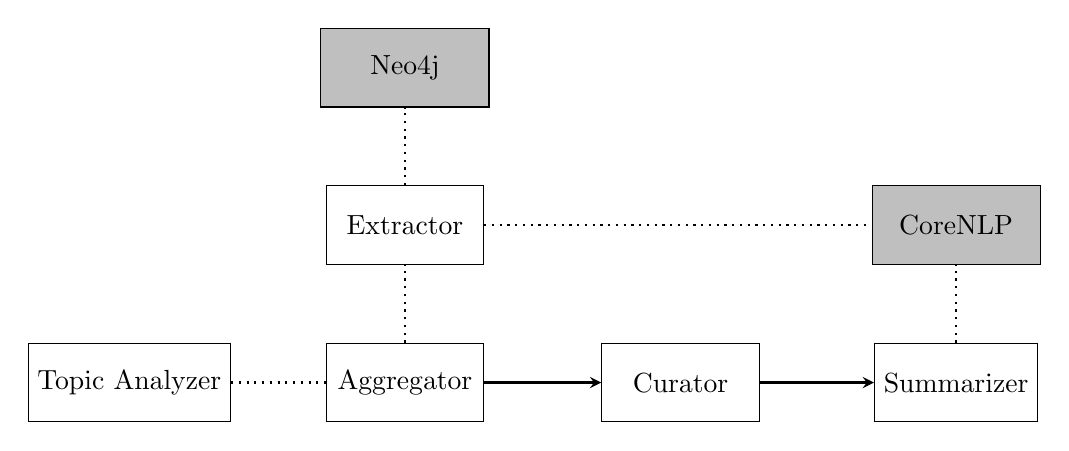
\begin{tikzpicture}[node distance=3.5cm]
      \node (agg) [service] {Aggregator};
      \node (top) [service, left of=agg] {Topic Analyzer};
      \node (ext) [service, above of=agg, yshift=-1.5cm] {Extractor};
      \node (cur) [service, right of=agg] {Curator};
      \node (sum) [service, right of=cur] {Summarizer};
      \node (cor) [extservice, above of=sum, yshift=-1.5cm] {CoreNLP};
      \node (neo) [extservice, above of=ext, yshift=-1.5cm] {Neo4j};

      \draw [flow] (agg) -- (cur);
      \draw [flow] (cur) -- (sum);
      \draw[dotted] [depends] (agg) -- (ext);
      \draw[dotted] [depends] (ext) -- (neo);
      \draw[dotted] [depends] (ext) -- (cor);
      \draw[dotted] [depends] (sum) -- (cor);
      \draw[dotted] [depends] (top) -- (agg);
    \end{tikzpicture}
    \caption{\\Architecture Diagram. Arrows represent the pipeline data flow; dotted lines represent dependencies.}
    \label{fig:arch-dia}
  \end{figure}

  Figure \ref{fig:arch-dia} shows a high-level overview of the various modules and how these make up the analysis pipeline. Points for all posts in the source text are gathered by the \textit{Aggregator}, these are filtered and cleaned by the \textit{Curator}. Finally curated points are used to generate a summary by the \textit{Summarizer}.

  Before source text can be analyzed it must be cleaned for invalid characters. Posts in a discussion begin as single text files, these are loaded and transformed into JSON files that preserve their index and valid UTF-8 content. The \textit{Aggregator} loads these JSON post files to extract the points made in the discussion.

  The \textit{Aggregator} loads all the JSON posts for the selected discussion. Before extracting points for each in turn it uses the text from all the posts (representing the discussion) to collect a list of topic words from the \textit{Topic Analyzer}. For each post in turn the text and topics\footnote{Only sentences containing a topic word care analyzed for points to reduce processing time.} are submitted to the \textit{Extractor}. This carries out the point extraction process using for each sentence in the post using both the CoreNLP dependency parser and Neo4j datastore - this is described in detail in Chapter \ref{chap:point-extraction}. All extracted points for all posts are saved to disk. A modern, mid-range computer can complete 150,000 words spread across 2300 posts in around 10 minutes, this is the slowest stage of the analysis pipeline.

  While points must come from a sentence containing a topic word, at this stage points are still largely unfiltered. The \textit{Curator}, a short program to filter and re-format points makes a series of transformations on points such as merging pronouns under a single \texttt{PERSON} label. Patterns for low-quality points are also encoded at this stage, for example: the \texttt{PERSON.nsubj be.verb sure.adj} point pattern that comes from every ``\textit{I'm sure}''. These transformations and rejections are applied to the list of points and a refined version is saved for use at the next stage (see Chapter \ref{chap:point-curation}).

  The \textit{Summarizer} is the final stage in the pipeline. Given a list of curated points, this module groups common points into the different summary sections. Sections are filled using points that have not been used and are suitable for the current group. Once a point has been used in section, it cannot be used again. This module must also choose an extract to display for each point. The point \texttt{abortion.nsubj be.verb right.dobj} occurs many times in the discussion and a single occurrence to represent this must be selected. This process makes use of the CoreNLP module again to request a dependency parse used in rating the quality of extracts. Selected extracts are formatted and used as text seen in summaries.

  The \texttt{Summarizer} formats the grouped extracts for selected point patterns as summary HTML files. This is the end of the pipeline - possibilities for further work are discussed in Chapter \ref{chap:conclusion}.

  A monolithic architecture was avoided due to processing time required at each stage. Running the entire process when making adjustments at the final stage was not feasible. Currently stages in the pipeline must be run manually however this is trivial to automate. The process for using the pipeline has been outlined in the Maintenance Manual in Appendix \ref{app:maintain}.

  The following chapters build on this technical overview and give more detail on the intricacies of the analysis performed by each module.
